\usetikzlibrary{arrows.meta,calc}
% Source: 2006 Sichuan liberal Q15, original_01.pdf p.1 (printed p.334).
% Ellipse x^2/25+y^2/16=1; AB is the major axis divided into 8 equal parts;
% P_1,...,P_7 are the upper intersections of the perpendiculars with the ellipse;
% F is the left focus (-3,0).  No numeric ticks are shown in the source.
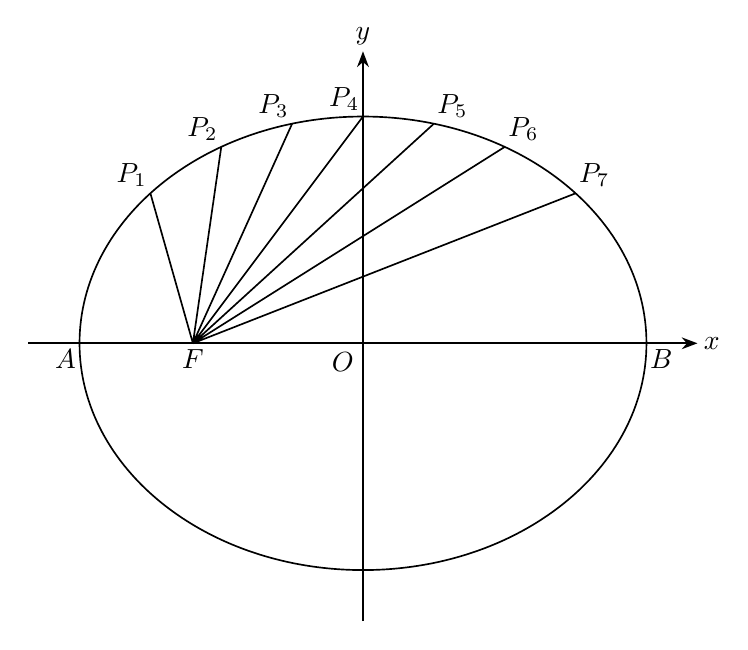
\begin{tikzpicture}[x=0.72cm,y=0.72cm,line width=.6pt,font=\normalsize,>=Stealth]
  \coordinate (O) at (0,0);
  \coordinate (A) at (-5,0);
  \coordinate (B) at (5,0);
  \coordinate (F) at (-3,0);
  \coordinate (P1) at (-3.75,2.6458);
  \coordinate (P2) at (-2.5,3.4641);
  \coordinate (P3) at (-1.25,3.8730);
  \coordinate (P4) at (0,4);
  \coordinate (P5) at (1.25,3.8730);
  \coordinate (P6) at (2.5,3.4641);
  \coordinate (P7) at (3.75,2.6458);
  \draw (O) ellipse [x radius=5,y radius=4];
  \draw[->] (-5.9,0) -- (5.9,0) node[right,inner sep=0pt,xshift=2pt] {$x$};
  \draw[->] (0,-4.9) -- (0,5.15) node[above,inner sep=0pt,yshift=2pt] {$y$};
  \draw (F)--(P1) (F)--(P2) (F)--(P3) (F)--(P4)
        (F)--(P5) (F)--(P6) (F)--(P7);
  \node[below left,inner sep=0pt,xshift=-1pt,yshift=-2pt] at (A) {$A$};
  \node[below right,inner sep=0pt,xshift=1pt,yshift=-2pt] at (B) {$B$};
  \node[below,inner sep=0pt,yshift=-2pt] at (F) {$F$};
  \node[below left,inner sep=3pt] at (O) {$O$};
  \node[above left,inner sep=0pt,xshift=-1pt,yshift=2pt] at (P1) {$P_{1}$};
  \node[above left,inner sep=0pt,xshift=-1pt,yshift=2pt] at (P2) {$P_{2}$};
  \node[above left,inner sep=0pt,xshift=-1pt,yshift=2pt] at (P3) {$P_{3}$};
  \node[above left,inner sep=0pt,xshift=-1pt,yshift=2pt] at (P4) {$P_{4}$};
  \node[above right,inner sep=0pt,xshift=1pt,yshift=2pt] at (P5) {$P_{5}$};
  \node[above right,inner sep=0pt,xshift=1pt,yshift=2pt] at (P6) {$P_{6}$};
  \node[above right,inner sep=0pt,xshift=1pt,yshift=2pt] at (P7) {$P_{7}$};
\end{tikzpicture}
